
\documentclass[journal]{IEEEtran}

% Some very useful LaTeX packages include:
% (uncomment the ones you want to load)

% *** MISC UTILITY PACKAGES ***
%
%\usepackage{ifpdf}
% Heiko Oberdiek's ifpdf.sty is very useful if you need conditional
% compilation based on whether the output is pdf or dvi.
% usage:
% \ifpdf
%   % pdf code
% \else
%   % dvi code
% \fi
% The latest version of ifpdf.sty can be obtained from:
% http://www.ctan.org/tex-archive/macros/latex/contrib/oberdiek/
% Also, note that IEEEtran.cls V1.7 and later provides a builtin
% \ifCLASSINFOpdf conditional that works the same way.
% When switching from latex to pdflatex and vice-versa, the compiler may
% have to be run twice to clear warning/error messages.

% *** CITATION PACKAGES ***
%
%\usepackage{cite}
% cite.sty was written by Donald Arseneau
% V1.6 and later of IEEEtran pre-defines the format of the cite.sty package
% \cite{} output to follow that of IEEE. Loading the cite package will
% result in citation numbers being automatically sorted and properly
% "compressed/ranged". e.g., [1], [9], [2], [7], [5], [6] without using
% cite.sty will become [1], [2], [5]--[7], [9] using cite.sty. cite.sty's
% \cite will automatically add leading space, if needed. Use cite.sty's
% noadjust option (cite.sty V3.8 and later) if you want to turn this off
% such as if a citation ever needs to be enclosed in parenthesis.
% cite.sty is already installed on most LaTeX systems. Be sure and use
% version 5.0 (2009-03-20) and later if using hyperref.sty.
% The latest version can be obtained at:
% http://www.ctan.org/tex-archive/macros/latex/contrib/cite/
% The documentation is contained in the cite.sty file itself.

% *** GRAPHICS RELATED PACKAGES ***
%
\ifCLASSINFOpdf
  \usepackage[pdftex]{graphicx}
  % declare the path(s) where your graphic files are
  \graphicspath{{../imagenes/}}
  % and their extensions so you won't have to specify these with
  % every instance of \includegraphics
  \DeclareGraphicsExtensions{.png}
\else
  % or other class option (dvipsone, dvipdf, if not using dvips). graphicx
  % will default to the driver specified in the system graphics.cfg if no
  % driver is specified.
  % \usepackage[dvips]{graphicx}
  % declare the path(s) where your graphic files are
  % \graphicspath{{../eps/}}
  % and their extensions so you won't have to specify these with
  % every instance of \includegraphics
  % \DeclareGraphicsExtensions{.eps}
\fi
% graphicx was written by David Carlisle and Sebastian Rahtz. It is
% required if you want graphics, photos, etc. graphicx.sty is already
% installed on most LaTeX systems. The latest version and documentation
% can be obtained at: 
% http://www.ctan.org/tex-archive/macros/latex/required/graphics/
% Another good source of documentation is "Using Imported Graphics in
% LaTeX2e" by Keith Reckdahl which can be found at:
% http://www.ctan.org/tex-archive/info/epslatex/
%
% latex, and pdflatex in dvi mode, support graphics in encapsulated
% postscript (.eps) format. pdflatex in pdf mode supports graphics
% in .pdf, .jpeg, .png and .mps (metapost) formats. Users should ensure
% that all non-photo figures use a vector format (.eps, .pdf, .mps) and
% not a bitmapped formats (.jpeg, .png). IEEE frowns on bitmapped formats
% which can result in "jaggedy"/blurry rendering of lines and letters as
% well as large increases in file sizes.
%
% You can find documentation about the pdfTeX application at:
% http://www.tug.org/applications/pdftex

% *** MATH PACKAGES ***
%
\usepackage[cmex10]{amsmath}
% A popular package from the American Mathematical Society that provides
% many useful and powerful commands for dealing with mathematics. If using
% it, be sure to load this package with the cmex10 option to ensure that
% only type 1 fonts will utilized at all point sizes. Without this option,
% it is possible that some math symbols, particularly those within
% footnotes, will be rendered in bitmap form which will result in a
% document that can not be IEEE Xplore compliant!
%
% Also, note that the amsmath package sets \interdisplaylinepenalty to 10000
% thus preventing page breaks from occurring within multiline equations. Use:
\interdisplaylinepenalty=2500
% after loading amsmath to restore such page breaks as IEEEtran.cls normally
% does. amsmath.sty is already installed on most LaTeX systems. The latest
% version and documentation can be obtained at:
% http://www.ctan.org/tex-archive/macros/latex/required/amslatex/math/

% *** SPECIALIZED LIST PACKAGES ***
%
%\usepackage{algorithmic}
% algorithmic.sty was written by Peter Williams and Rogerio Brito.
% This package provides an algorithmic environment fo describing algorithms.
% You can use the algorithmic environment in-text or within a figure
% environment to provide for a floating algorithm. Do NOT use the algorithm
% floating environment provided by algorithm.sty (by the same authors) or
% algorithm2e.sty (by Christophe Fiorio) as IEEE does not use dedicated
% algorithm float types and packages that provide these will not provide
% correct IEEE style captions. The latest version and documentation of
% algorithmic.sty can be obtained at:
% http://www.ctan.org/tex-archive/macros/latex/contrib/algorithms/
% There is also a support site at:
% http://algorithms.berlios.de/index.html
% Also of interest may be the (relatively newer and more customizable)
% algorithmicx.sty package by Szasz Janos:
% http://www.ctan.org/tex-archive/macros/latex/contrib/algorithmicx/

% *** ALIGNMENT PACKAGES ***
%
%\usepackage{array}
% Frank Mittelbach's and David Carlisle's array.sty patches and improves
% the standard LaTeX2e array and tabular environments to provide better
% appearance and additional user controls. As the default LaTeX2e table
% generation code is lacking to the point of almost being broken with
% respect to the quality of the end results, all users are strongly
% advised to use an enhanced (at the very least that provided by array.sty)
% set of table tools. array.sty is already installed on most systems. The
% latest version and documentation can be obtained at:
% http://www.ctan.org/tex-archive/macros/latex/required/tools/

% IEEEtran contains the IEEEeqnarray family of commands that can be used to
% generate multiline equations as well as matrices, tables, etc., of high
% quality.

% *** SUBFIGURE PACKAGES ***
\ifCLASSOPTIONcompsoc
 \usepackage[caption=false,font=normalsize,labelfont=sf,textfont=sf]{subfig}
\else
 \usepackage[caption=false,font=footnotesize]{subfig}
\fi
% subfig.sty, written by Steven Douglas Cochran, is the modern replacement
% for subfigure.sty, the latter of which is no longer maintained and is
% incompatible with some LaTeX packages including fixltx2e. However,
% subfig.sty requires and automatically loads Axel Sommerfeldt's caption.sty
% which will override IEEEtran.cls' handling of captions and this will result
% in non-IEEE style figure/table captions. To prevent this problem, be sure
% and invoke subfig.sty's "caption=false" package option (available since
% subfig.sty version 1.3, 2005/06/28) as this is will preserve IEEEtran.cls
% handling of captions.
% Note that the Computer Society format requires a larger sans serif font
% than the serif footnote size font used in traditional IEEE formatting
% and thus the need to invoke different subfig.sty package options depending
% on whether compsoc mode has been enabled.
%
% The latest version and documentation of subfig.sty can be obtained at:
% http://www.ctan.org/tex-archive/macros/latex/contrib/subfig/

% *** FLOAT PACKAGES ***
%
%\usepackage{fixltx2e}
% fixltx2e, the successor to the earlier fix2col.sty, was written by
% Frank Mittelbach and David Carlisle. This package corrects a few problems
% in the LaTeX2e kernel, the most notable of which is that in current
% LaTeX2e releases, the ordering of single and double column floats is not
% guaranteed to be preserved. Thus, an unpatched LaTeX2e can allow a
% single column figure to be placed prior to an earlier double column
% figure. The latest version and documentation can be found at:
% http://www.ctan.org/tex-archive/macros/latex/base/

%\usepackage{stfloats}
% stfloats.sty was written by Sigitas Tolusis. This package gives LaTeX2e
% the ability to do double column floats at the bottom of the page as well
% as the top. (e.g., "\begin{figure*}[!b]" is not normally possible in
% LaTeX2e). It also provides a command:
%\fnbelowfloat
% to enable the placement of footnotes below bottom floats (the standard
% LaTeX2e kernel puts them above bottom floats). This is an invasive package
% which rewrites many portions of the LaTeX2e float routines. It may not work
% with other packages that modify the LaTeX2e float routines. The latest
% version and documentation can be obtained at:
% http://www.ctan.org/tex-archive/macros/latex/contrib/sttools/
% Do not use the stfloats baselinefloat ability as IEEE does not allow
% \baselineskip to stretch. Authors submitting work to the IEEE should note
% that IEEE rarely uses double column equations and that authors should try
% to avoid such use. Do not be tempted to use the cuted.sty or midfloat.sty
% packages (also by Sigitas Tolusis) as IEEE does not format its papers in
% such ways.
% Do not attempt to use stfloats with fixltx2e as they are incompatible.
% Instead, use Morten Hogholm'a dblfloatfix which combines the features
% of both fixltx2e and stfloats:
%
% \usepackage{dblfloatfix}
% The latest version can be found at:
% http://www.ctan.org/tex-archive/macros/latex/contrib/dblfloatfix/

%\ifCLASSOPTIONcaptionsoff
%  \usepackage[nomarkers]{endfloat}
% \let\MYoriglatexcaption\caption
% \renewcommand{\caption}[2][\relax]{\MYoriglatexcaption[#2]{#2}}
%\fi
% endfloat.sty was written by James Darrell McCauley, Jeff Goldberg and 
% Axel Sommerfeldt. This package may be useful when used in conjunction with 
% IEEEtran.cls'  captionsoff option. Some IEEE journals/societies require that
% submissions have lists of figures/tables at the end of the paper and that
% figures/tables without any captions are placed on a page by themselves at
% the end of the document. If needed, the draftcls IEEEtran class option or
% \CLASSINPUTbaselinestretch interface can be used to increase the line
% spacing as well. Be sure and use the nomarkers option of endfloat to
% prevent endfloat from "marking" where the figures would have been placed
% in the text. The two hack lines of code above are a slight modification of
% that suggested by in the endfloat docs (section 8.4.1) to ensure that
% the full captions always appear in the list of figures/tables - even if
% the user used the short optional argument of \caption[]{}.
% IEEE papers do not typically make use of \caption[]'s optional argument,
% so this should not be an issue. A similar trick can be used to disable
% captions of packages such as subfig.sty that lack options to turn off
% the subcaptions:
% For subfig.sty:
% \let\MYorigsubfloat\subfloat
% \renewcommand{\subfloat}[2][\relax]{\MYorigsubfloat[]{#2}}
% However, the above trick will not work if both optional arguments of
% the \subfloat command are used. Furthermore, there needs to be a
% description of each subfigure *somewhere* and endfloat does not add
% subfigure captions to its list of figures. Thus, the best approach is to
% avoid the use of subfigure captions (many IEEE journals avoid them anyway)
% and instead reference/explain all the subfigures within the main caption.
% The latest version of endfloat.sty and its documentation can obtained at:
% http://www.ctan.org/tex-archive/macros/latex/contrib/endfloat/
%
% The IEEEtran \ifCLASSOPTIONcaptionsoff conditional can also be used
% later in the document, say, to conditionally put the References on a 
% page by themselves.

% *** PDF, URL AND HYPERLINK PACKAGES ***
%
%\usepackage{url}
% url.sty was written by Donald Arseneau. It provides better support for
% handling and breaking URLs. url.sty is already installed on most LaTeX
% systems. The latest version and documentation can be obtained at:
% http://www.ctan.org/tex-archive/macros/latex/contrib/url/
% Basically, \url{my_url_here}.

% *** Do not adjust lengths that control margins, column widths, etc. ***
% *** Do not use packages that alter fonts (such as pslatex).         ***
% There should be no need to do such things with IEEEtran.cls V1.6 and later.
% (Unless specifically asked to do so by the journal or conference you plan
% to submit to, of course. )

\usepackage[utf8]{inputenc}
\usepackage{svg}

\usepackage{tikz}
\usetikzlibrary{shapes.misc, shapes.geometric,
    shapes.arrows, decorations.pathmorphing}
\usetikzlibrary{matrix, chains, scopes, positioning, arrows, fit, graphs}

\tikzset{
    every new ->/.style={shorten >=1pt},
    graphs/every graph/.style={edges=rounded corners},
    bloque/.style={rectangle, minimum height=2.5em, minimum width=3em, draw=black},
    suma/.style={draw, circle, node distance=1cm},
    ganancia/.style={draw, shape border rotate=-90, regular polygon,
        regular polygon sides=3, node distance=0.8cm,},
    input/.style={coordinate},
    output/.style={coordinate},
    conexion/.style={coordinate}}

% correct bad hyphenation here
\hyphenation{op-tical net-works semi-conduc-tor}


\begin{document}
%
% paper title
% Titles are generally capitalized except for words such as a, an, and, as,
% at, but, by, for, in, nor, of, on, or, the, to and up, which are usually
% not capitalized unless they are the first or last word of the title.
% Linebreaks \\ can be used within to get better formatting as desired.
% Do not put math or special symbols in the title.
\title{A Working Example of an Adaptive Controller
    With the Slotine Li Algorithm}

%
% author names and IEEE memberships
% note positions of commas and nonbreaking spaces ( ~ ) LaTeX will not break
% a structure at a ~ so this keeps an author's name from being broken across
% two lines.
% use \thanks{} to gain access to the first footnote area
% a separate \thanks must be used for each paragraph as LaTeX2e's \thanks
% was not built to handle multiple paragraphs
%

\author{Roberto~Cadena~Vega% <-this % stops a space
\thanks{R. Cadena Vega is a student of the Department of Automatic Control,
    CINVESTAV-IPN, México, e-mail:(rcadena@ctrl.cinvestav.mx).}% <-this % stops a space
\thanks{Manuscript delivered April 20, 2015}}

% note the % following the last \IEEEmembership and also \thanks - 
% these prevent an unwanted space from occurring between the last author name
% and the end of the author line. i.e., if you had this:
% 
% \author{....lastname \thanks{...} \thanks{...} }
%                     ^------------^------------^----Do not want these spaces!
%
% a space would be appended to the last name and could cause every name on that
% line to be shifted left slightly. This is one of those "LaTeX things". For
% instance, "\textbf{A} \textbf{B}" will typeset as "A B" not "AB". To get
% "AB" then you have to do: "\textbf{A}\textbf{B}"
% \thanks is no different in this regard, so shield the last } of each \thanks
% that ends a line with a % and do not let a space in before the next \thanks.
% Spaces after \IEEEmembership other than the last one are OK (and needed) as
% you are supposed to have spaces between the names. For what it is worth,
% this is a minor point as most people would not even notice if the said evil
% space somehow managed to creep in.

% The paper headers
\markboth{Introduction to Robotics Paper}%
{Shell \MakeLowercase{\textit{et al.}}: Bare Demo of IEEEtran.cls for Journals}
% The only time the second header will appear is for the odd numbered pages
% after the title page when using the twoside option.
% 
% *** Note that you probably will NOT want to include the author's ***
% *** name in the headers of peer review papers.                   ***
% You can use \ifCLASSOPTIONpeerreview for conditional compilation here if
% you desire.

% make the title area
\maketitle

% As a general rule, do not put math, special symbols or citations
% in the abstract or keywords.
\begin{abstract}
The abstract goes here.
\end{abstract}

% For peer review papers, you can put extra information on the cover
% page as needed:
% \ifCLASSOPTIONpeerreview
% \begin{center} \bfseries EDICS Category: 3-BBND \end{center}
% \fi
%
% For peerreview papers, this IEEEtran command inserts a page break and
% creates the second title. It will be ignored for other modes.
% \IEEEpeerreviewmaketitle

\section{Introduction}
% The very first letter is a 2 line initial drop letter followed
% by the rest of the first word in caps.
% 
% form to use if the first word consists of a single letter:
% \IEEEPARstart{A}{demo} file is ....
% 
% form to use if you need the single drop letter followed by
% normal text (unknown if ever used by IEEE):
% \IEEEPARstart{A}{}demo file is ....
% 
% Some journals put the first two words in caps:
% \IEEEPARstart{T}{his demo} file is ....
% 
% Here we have the typical use of a "T" for an initial drop letter
% and "HIS" in caps to complete the first word.
\IEEEPARstart{T}{he} intention of this paper is to provide a simple implementation of the Slotine Li Algorithm to control a robotic manipulator with an adaptive control law.

\section{Preliminaries}

    \subsection{Servomechanism Model}

        The servomechanism used in this experiment consists of a DC motor with a brass disc on it's axis, connected to a power amplifier, so as to have a block diagram representation like the one in the figure~\ref{fig_servomodel}.

        \begin{figure*}[!t]
            \centering
            \begin{tikzpicture}[thick]
                \matrix[column sep=4mm, row sep=3mm]{
                    % Primera fila
                    & \node (c1)[conexion]{}; & & \node(neg)[bloque]{$-K_C$}; & & & \node (c2)[conexion]{}; & & & & & \\
                    % Segunda fila
                    \node (ent) {$u$}; &
                    \node (sum1) [suma] {\tiny$+$}; &
                    \node (curgain) [ganancia] {$\beta$}; &
                    \node (amp) [bloque] {$K_A$}; &
                    \node (sum2) [suma] {\tiny$+$}; &
                    \node (electrico) [bloque] {$\frac{1}{L_a s + R_a}$}; &
                    \node (armcur) [conexion] {}; &
                    \node (gan1) [bloque] {$K$}; &
                    \node (mecanico) [bloque] {$\frac{1}{J_m s + B_m}$}; &
                    \node (vel) [conexion] {}; &
                    \node (integ) [bloque] {$\frac{1}{s}$}; &
                    \node (pos) {$q$}; \\
                    % Tercer fila
                    & & & & \node (c3)[conexion]{}; & & & \node(cem)[bloque]{$-K_B$}; & & \node (c4)[conexion]{}; & & \\};

                \graph{
                    (ent) -> (sum1) -> (curgain) -> (amp) -> (sum2) -> (electrico) -> (gan1) -> (mecanico) -> (integ) -> (pos);
                    (armcur) -- (c2) -> (neg) -- (c1) -> (sum1);
                    (vel) -- (c4) -> (cem) -- (c3) -> (sum2);};
            \end{tikzpicture}
            \caption{Servomechanism model}
            \label{fig_servomodel}
        \end{figure*}

        Where $\beta$ is the gain of the power amplifier because of the armature current feedback loop, $K_C$ is a pre amplification stage, $K$ is the current-torque relation, $Kb$ is related to the counter electromotive force. Let's consider a high gain in the power amplification stage due to the current feedback loop, we can simplify this model to a much more simpler one:

        \begin{equation}
            \ddot{q}(t) + a \dot{q}(t) = b u(t)
        \end{equation}

        \begin{figure}[!t]
            \begin{center}
                \begin{tikzpicture}[thick]
                    \matrix[column sep=5mm]{
                        \node (ent) {$u$}; &
                        \node (servo) [bloque] {$\frac{b}{s + a}$}; &
                        \node (integ) [bloque] {$\frac{1}{s}$}; &
                        \node (sal) {$q$}; \\};

                    \graph{(ent) -> (servo) -> (integ) -> (sal) ;};
                \end{tikzpicture}
            \end{center}
            \caption{Simplified servomechanism model}
            \label{fig_simpleservomodel}
        \end{figure}

        Where $a$ and $b$ are defined as:

        \begin{align}
            a &= \frac{B_m}{J_m} \\
            b &= \frac{K}{K_C J_m}
        \end{align}

        We consider $\beta$ of great magnitude, so that the time constant of the electric servomechanism is smaller than the mechanical one.
        
    \subsection{Parameter Identification}

        In previous works it has been stablished that the values of the constants $a$ and $b$ are:

        \begin{align}   
            a &= 0.45 \\
            b &= 31.0
        \end{align}

        So, when presented the results of the estimation of this parameters, they will be compared against this results.

    \subsection{Slotine Li Algorithm for Non-linear Robot Manipulators}

        The Slotine-Li algorithm for robotic manipulator considers a dynamic equation for the robot like:

        \begin{equation}
            H(q) \ddot{q} + C(q, \dot{q}) + g(q) = \tau
        \end{equation}

        Which can be rewritten like this:

        \begin{equation} \label{closedloopslotine}
            \tilde{H}(q) \ddot{q}_r + \tilde{C}(q, \dot{q}) \dot{q}_r + \tilde{g}(q) = Y(q, \dot{q}, \dot{q}_r, \ddot{q}_r) \tilde{a}
        \end{equation}

        Where $\hat{a}$ is the parameter estimated through the adaptation law, and $\hat{H}(q)$ is the matrix $H(q)$ substituted with the estimated parameter $\hat{a}$. More over, we define the error in the estimation of the parameter $\tilde{a} = a = \hat{a}$ and $Y$ only depends on dynamic parameters. The error in the estimation of the state of the system is defined as $\tilde{q}(t) = q(t) - q_d(t)$ and we define a new state as:

        \begin{equation}
            \dot{q}_r = \dot{q}_d - \Lambda \tilde{q}
        \end{equation}

        so that when we use the proposed control law:

        \begin{equation}
            \tau = \hat{H}(q) \ddot{q}_r + \hat{C}(q, \dot{q}) \dot{q}_r + \hat{g}(q) - K_D s
        \end{equation}

        with the adaptation law:

        \begin{equation}
            \dot{\hat{a}} = - \Gamma Y^T s
        \end{equation}

        $\Gamma$ being a constant positive definite matrix, and $s$ being defined as:

        \begin{equation}
            s = \dot{q} - \dot{q}_r = \dot{\tilde{q}} + \Lambda \tilde{q}
        \end{equation}

        the equation of the closed loop system will be as stated in~\ref{closedloopslotine}.

    % \begin{center}
    %     \begin{tikzpicture}[thick]
    %         \matrix[row sep=4mm, column sep=4mm]{
    %              & & \node (c1)[conexion]{}; & & \node (c2)[conexion]{}; & \\
    %              & & & \node (s1)[conexion]{}; & \node (c3)[conexion]{}; & \\
    %             \node (ent) {$u$}; &
    %             \node (alpha) [ganancia] {$\alpha$}; &
    %             \node (sum) [suma] {\tiny$+$}; &
    %             \node (s2) [bloque] {Servomechanism}; &
    %             \node (q) [conexion] {}; &
    %             \node (sal) {$q$}; \\
    %              & & & \node (s3)[conexion]{}; & & \\};

    %         \graph{
    %             (ent) -> (alpha) -> (sum) -> (s2);
    %             (s2) -> (sal);
    %             (s1) -- (c3) -- (c2) -- (c1) -> (sum);};
    %     \end{tikzpicture}
    % \end{center}

    \subsection{Trajectories Generation}
        The algorithm needs not only the signal for the trajectory to track, but the derivative and the second derivative, both of them can be acheived with a second order filter like the one in the figure.

        \begin{figure*}[!t]
            \centering
            \begin{tikzpicture}[thick]
                \matrix[column sep=4mm, row sep=3mm]{
                    % Primer fila
                    & & \node (c1)[conexion]{}; & \node(neg)[bloque]{$-1$}; & & & & & & & \node (c2)[conexion]{}; & \\
                    % Segunda fila
                    & & & & \node (c6)[conexion]{}; & & \node (gan2) [bloque]{$-2 \alpha$}; & \node (c5)[conexion]{}; & & & & \\
                    % Tercer fila
                    \node (qdi) {$q_d$}; &
                    \node (fil1) [bloque] {$\frac{\alpha}{s + \alpha}$}; &
                    \node (sum1) [suma] {\tiny$+$}; &
                    \node (gan1) [bloque] {$\alpha^2$}; &
                    \node (sum2) [suma] {\tiny$+$}; &
                    \node (qdpp) [conexion] {}; &
                    \node (int1) [bloque] {$\frac{1}{s}$}; &
                    \node (qdp1) [conexion] {}; &
                    \node (qdp2) [conexion] {}; &
                    \node (int2) [bloque] {$\frac{1}{s}$}; &
                    \node (qd1) [conexion] {}; &
                    \node (qdo) {$\hat{q}_d$}; \\
                    % Cuarta fila
                    & & & & & & & & \node (c4)[conexion]{}; & & & \node (qdpo) {$\dot{\hat{q}}_d$}; \\
                    % Quinta fila
                    & & & & & \node (c3)[conexion]{}; & & & & & & \node (qdppo) {$\ddot{\hat{q}}_d$}; \\};

                \graph{
                    (qdi) -> (fil1) -> (sum1) -> (gan1) -> (sum2) -- (qdpp) -> (int1) -- (qdp1) -- (qdp2) -> (int2) -- (qd1) -> (qdo);
                    (qd1) -- (c2) -> (neg) -- (c1) -> (sum1);
                    (qdp1)
                    (qdp2) -- (c4) -> (qdpo);
                    (qdpp) -- (c3) -> (qdppo);};
            \end{tikzpicture}
            \caption{Second order filter for trajectory generation}
            \label{fig_seorfilter}
        \end{figure*}

\section{Experiment Parameters}
    

\section{Experimental Results}
Subsection text here.

\begin{figure}[!t]
    \centering
    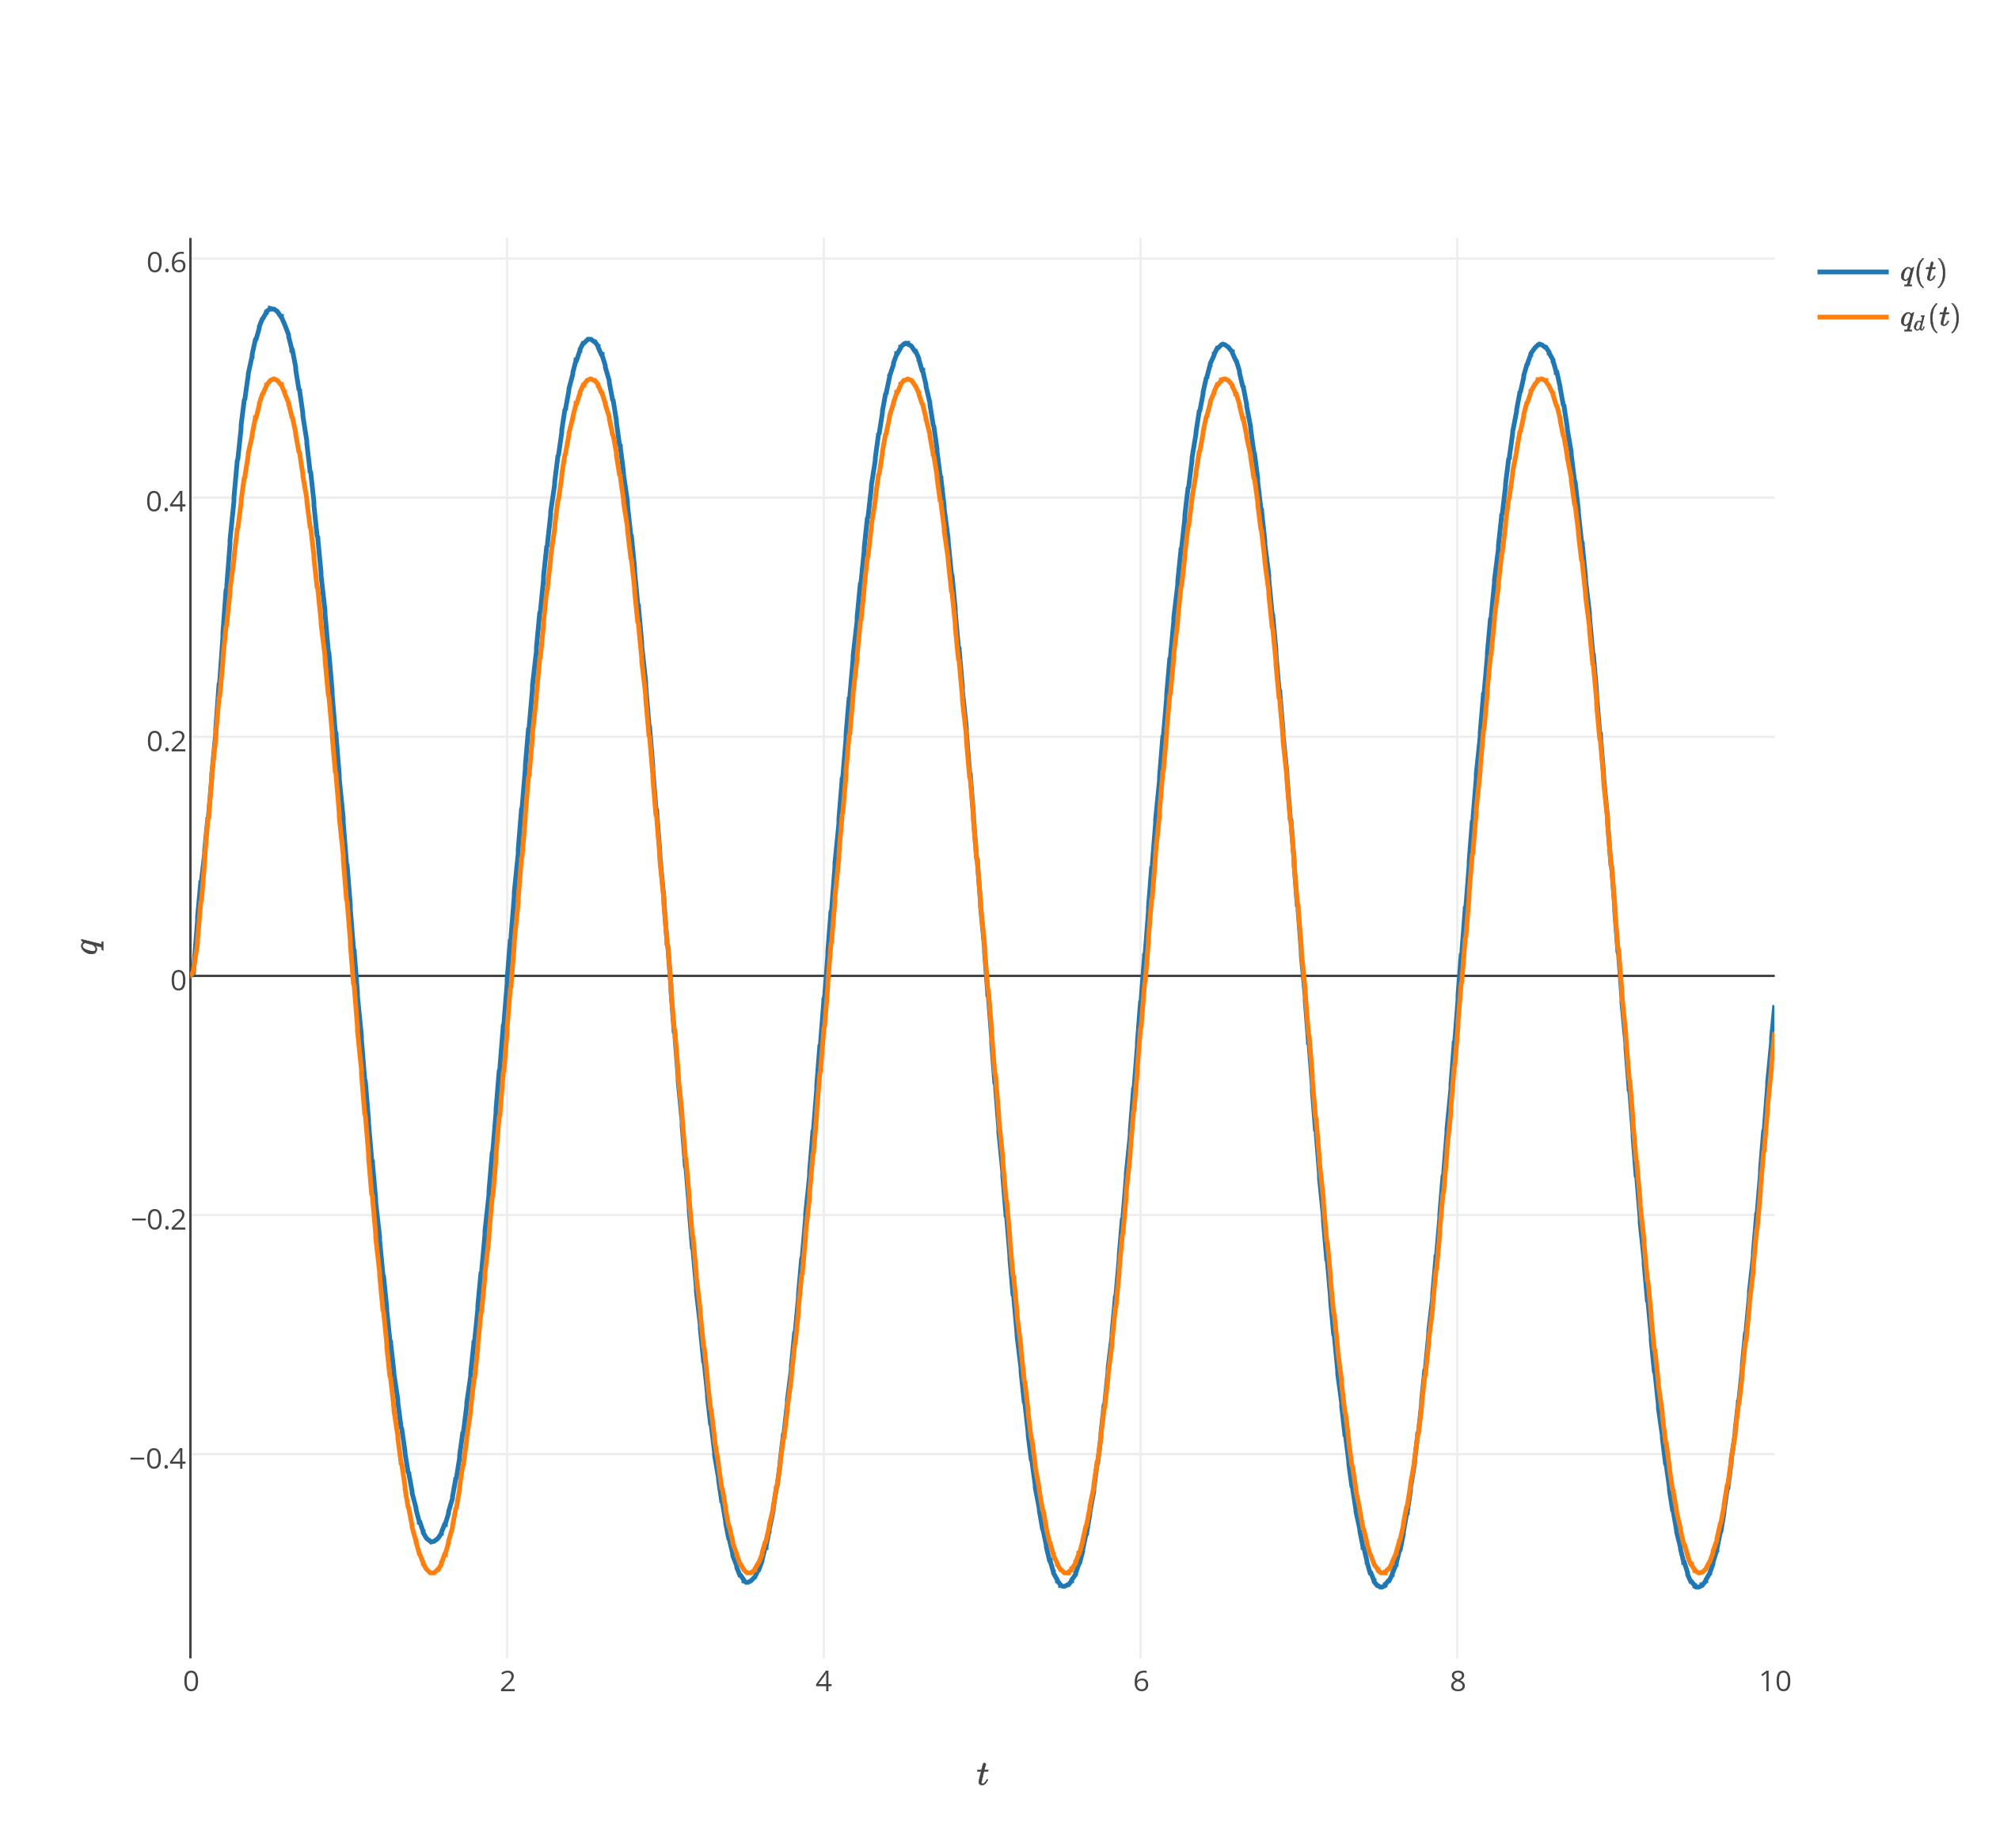
\includegraphics[width=7cm]{respuestatrayectoria}
    \caption{Servomechanism response against generated signal}
    \label{fig_respuesta}
\end{figure}

\begin{figure*}[!t]
    \centering
    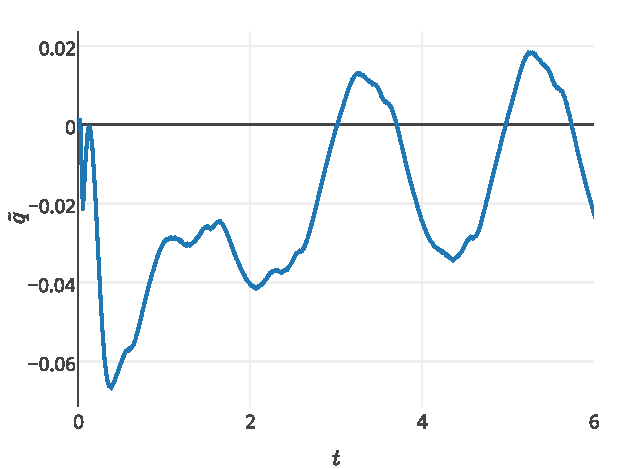
\includegraphics[width=\textwidth]{error}
    \caption{Error signal}
    \label{fig_error}
\end{figure*}

\begin{figure}[!t]
    \centering
    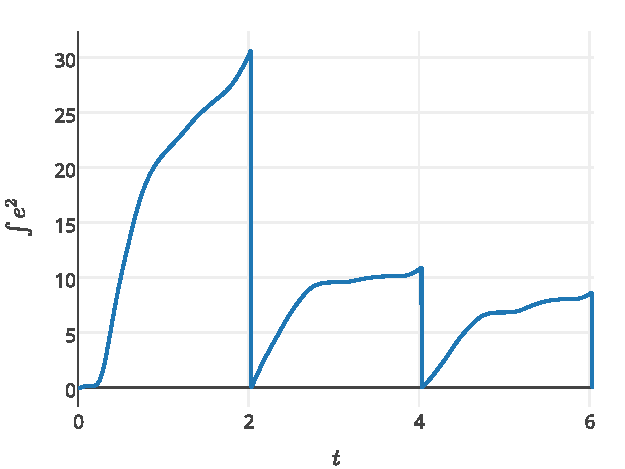
\includegraphics[width=7cm]{IEC}
    \caption{Integrated square error}
    \label{fig_iec}
\end{figure}

\begin{figure*}[!t]
    \centering
    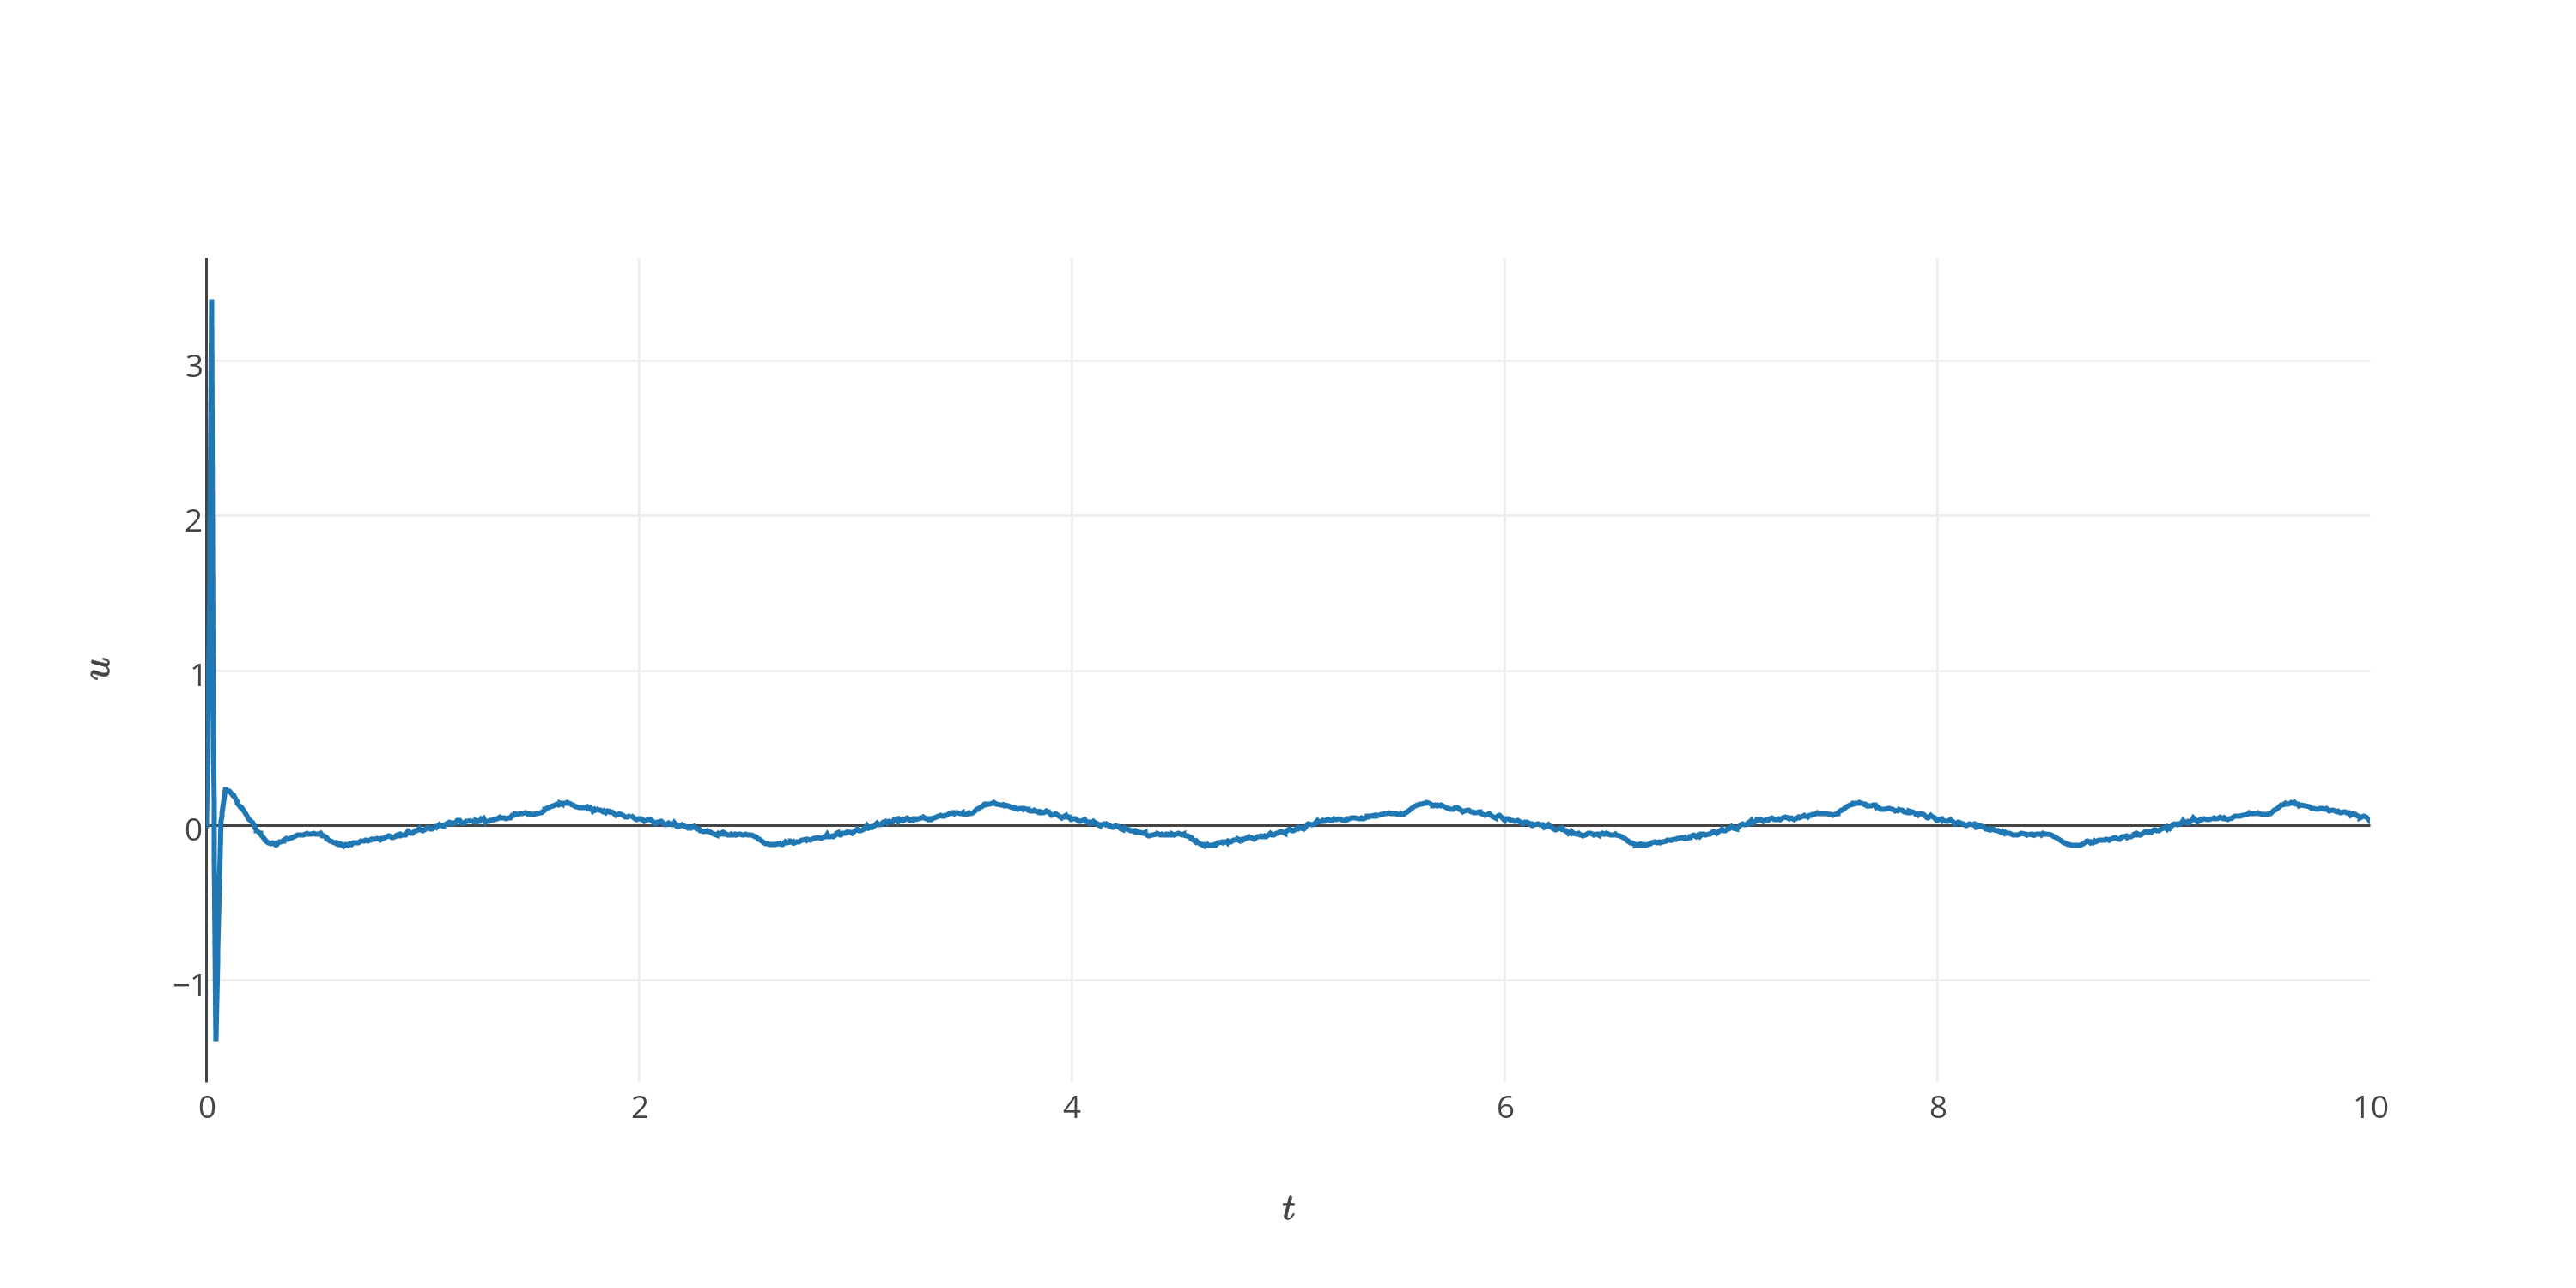
\includegraphics[width=\textwidth]{control}
    \caption{Control law signal}
    \label{fig_control}
\end{figure*}

\begin{figure}[!t]
    \centering
    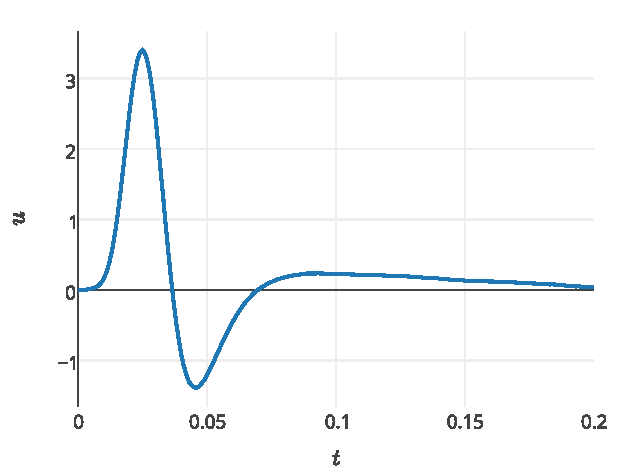
\includegraphics[width=7cm]{controlimpulse}
    \caption{Control signal first impulse}
    \label{fig_controlimpulse}
\end{figure}

\begin{figure*}[!t]
    \centering
    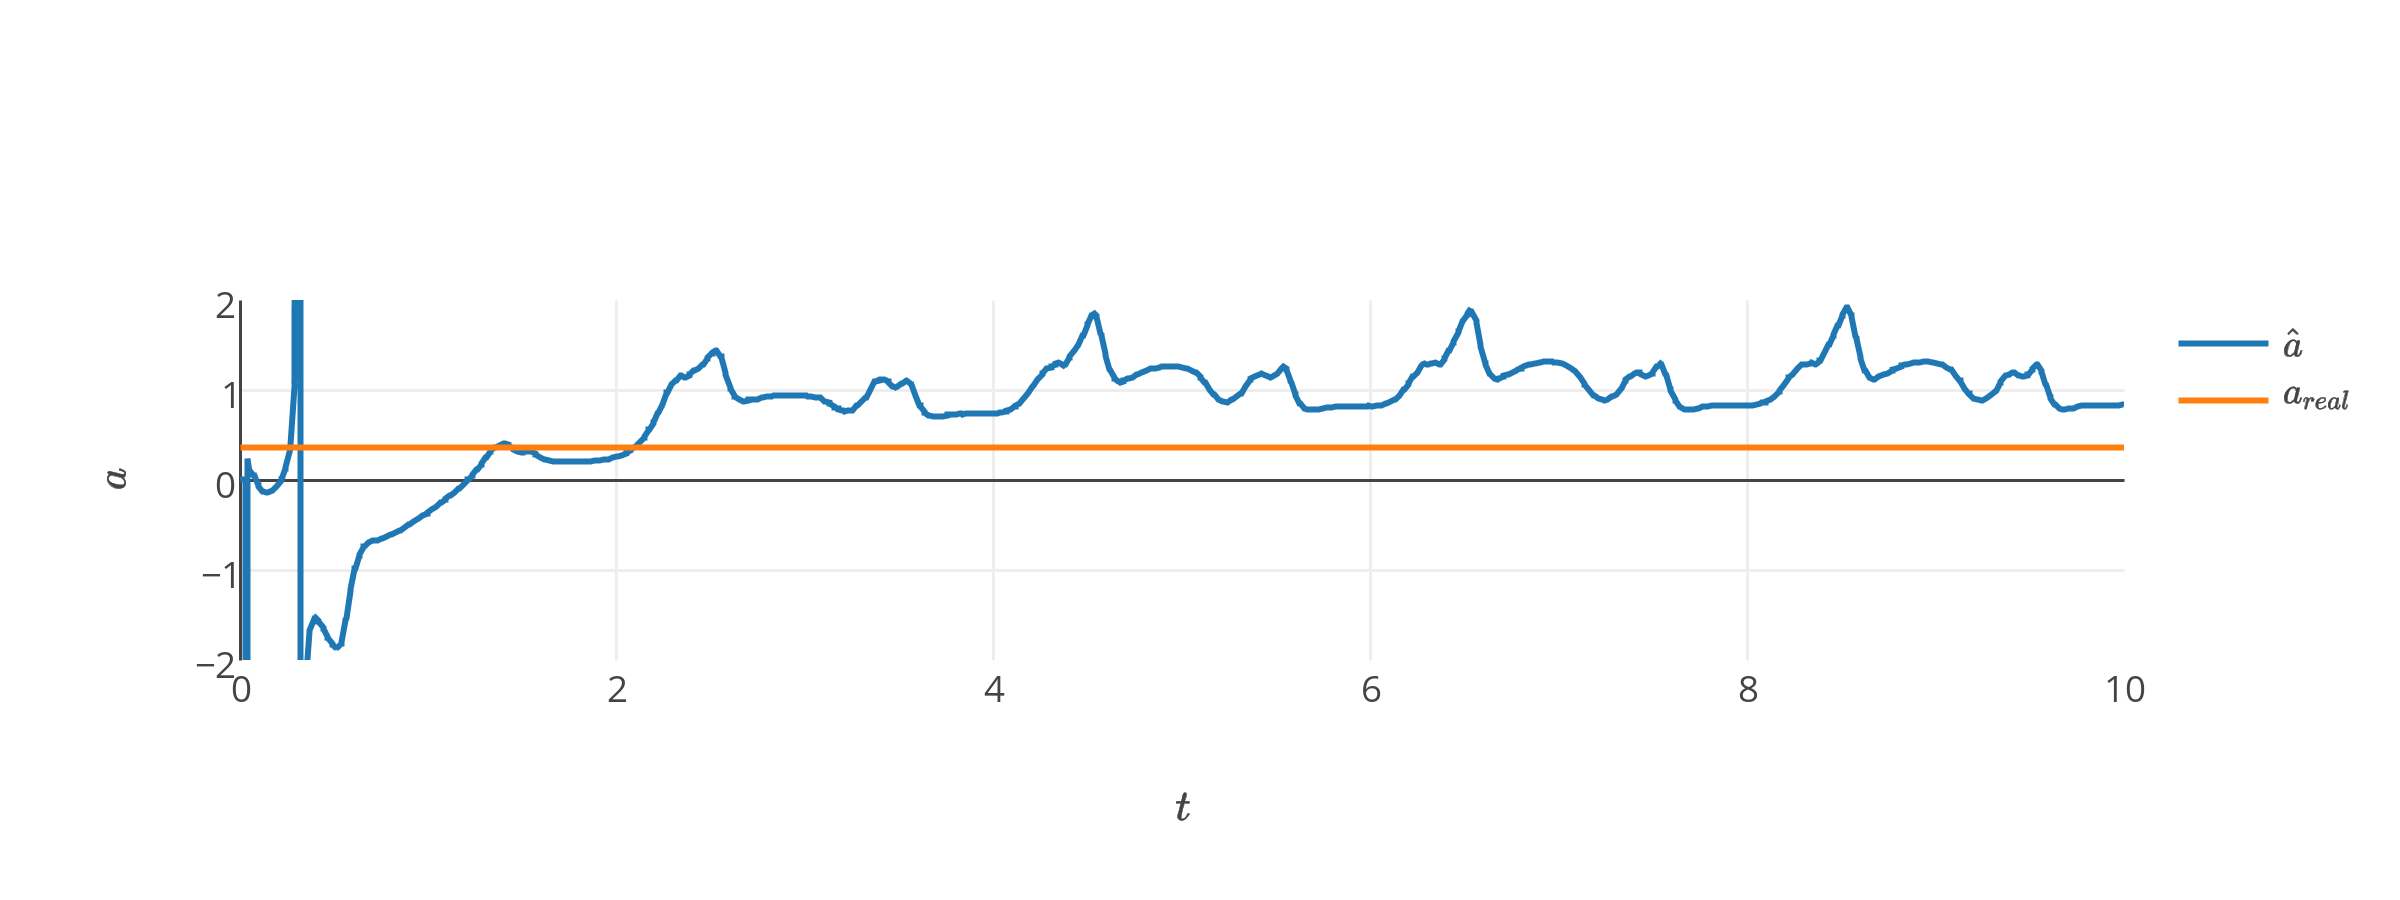
\includegraphics[width=\textwidth]{parametroa}
    \caption{Estimated signal of parameter a}
    \label{fig_parametroa}
\end{figure*}

\begin{figure*}[!t]
    \centering
    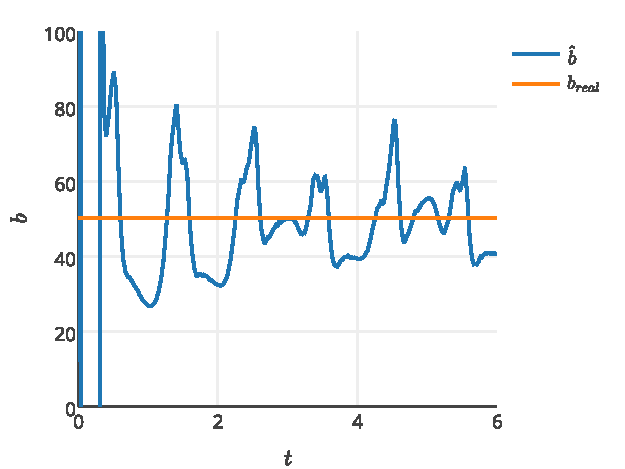
\includegraphics[width=\textwidth]{parametrob}
    \caption{Estimated signal of parameter b}
    \label{fig_parametrob}
\end{figure*}

% An example of a floating figure using the graphicx package.
% Note that \label must occur AFTER (or within) \caption.
% For figures, \caption should occur after the \includegraphics.
% Note that IEEEtran v1.7 and later has special internal code that
% is designed to preserve the operation of \label within \caption
% even when the captionsoff option is in effect. However, because
% of issues like this, it may be the safest practice to put all your
% \label just after \caption rather than within \caption{}.
%
% Reminder: the "draftcls" or "draftclsnofoot", not "draft", class
% option should be used if it is desired that the figures are to be
% displayed while in draft mode.
%
% \begin{figure*}[!t]
%     \centering
%     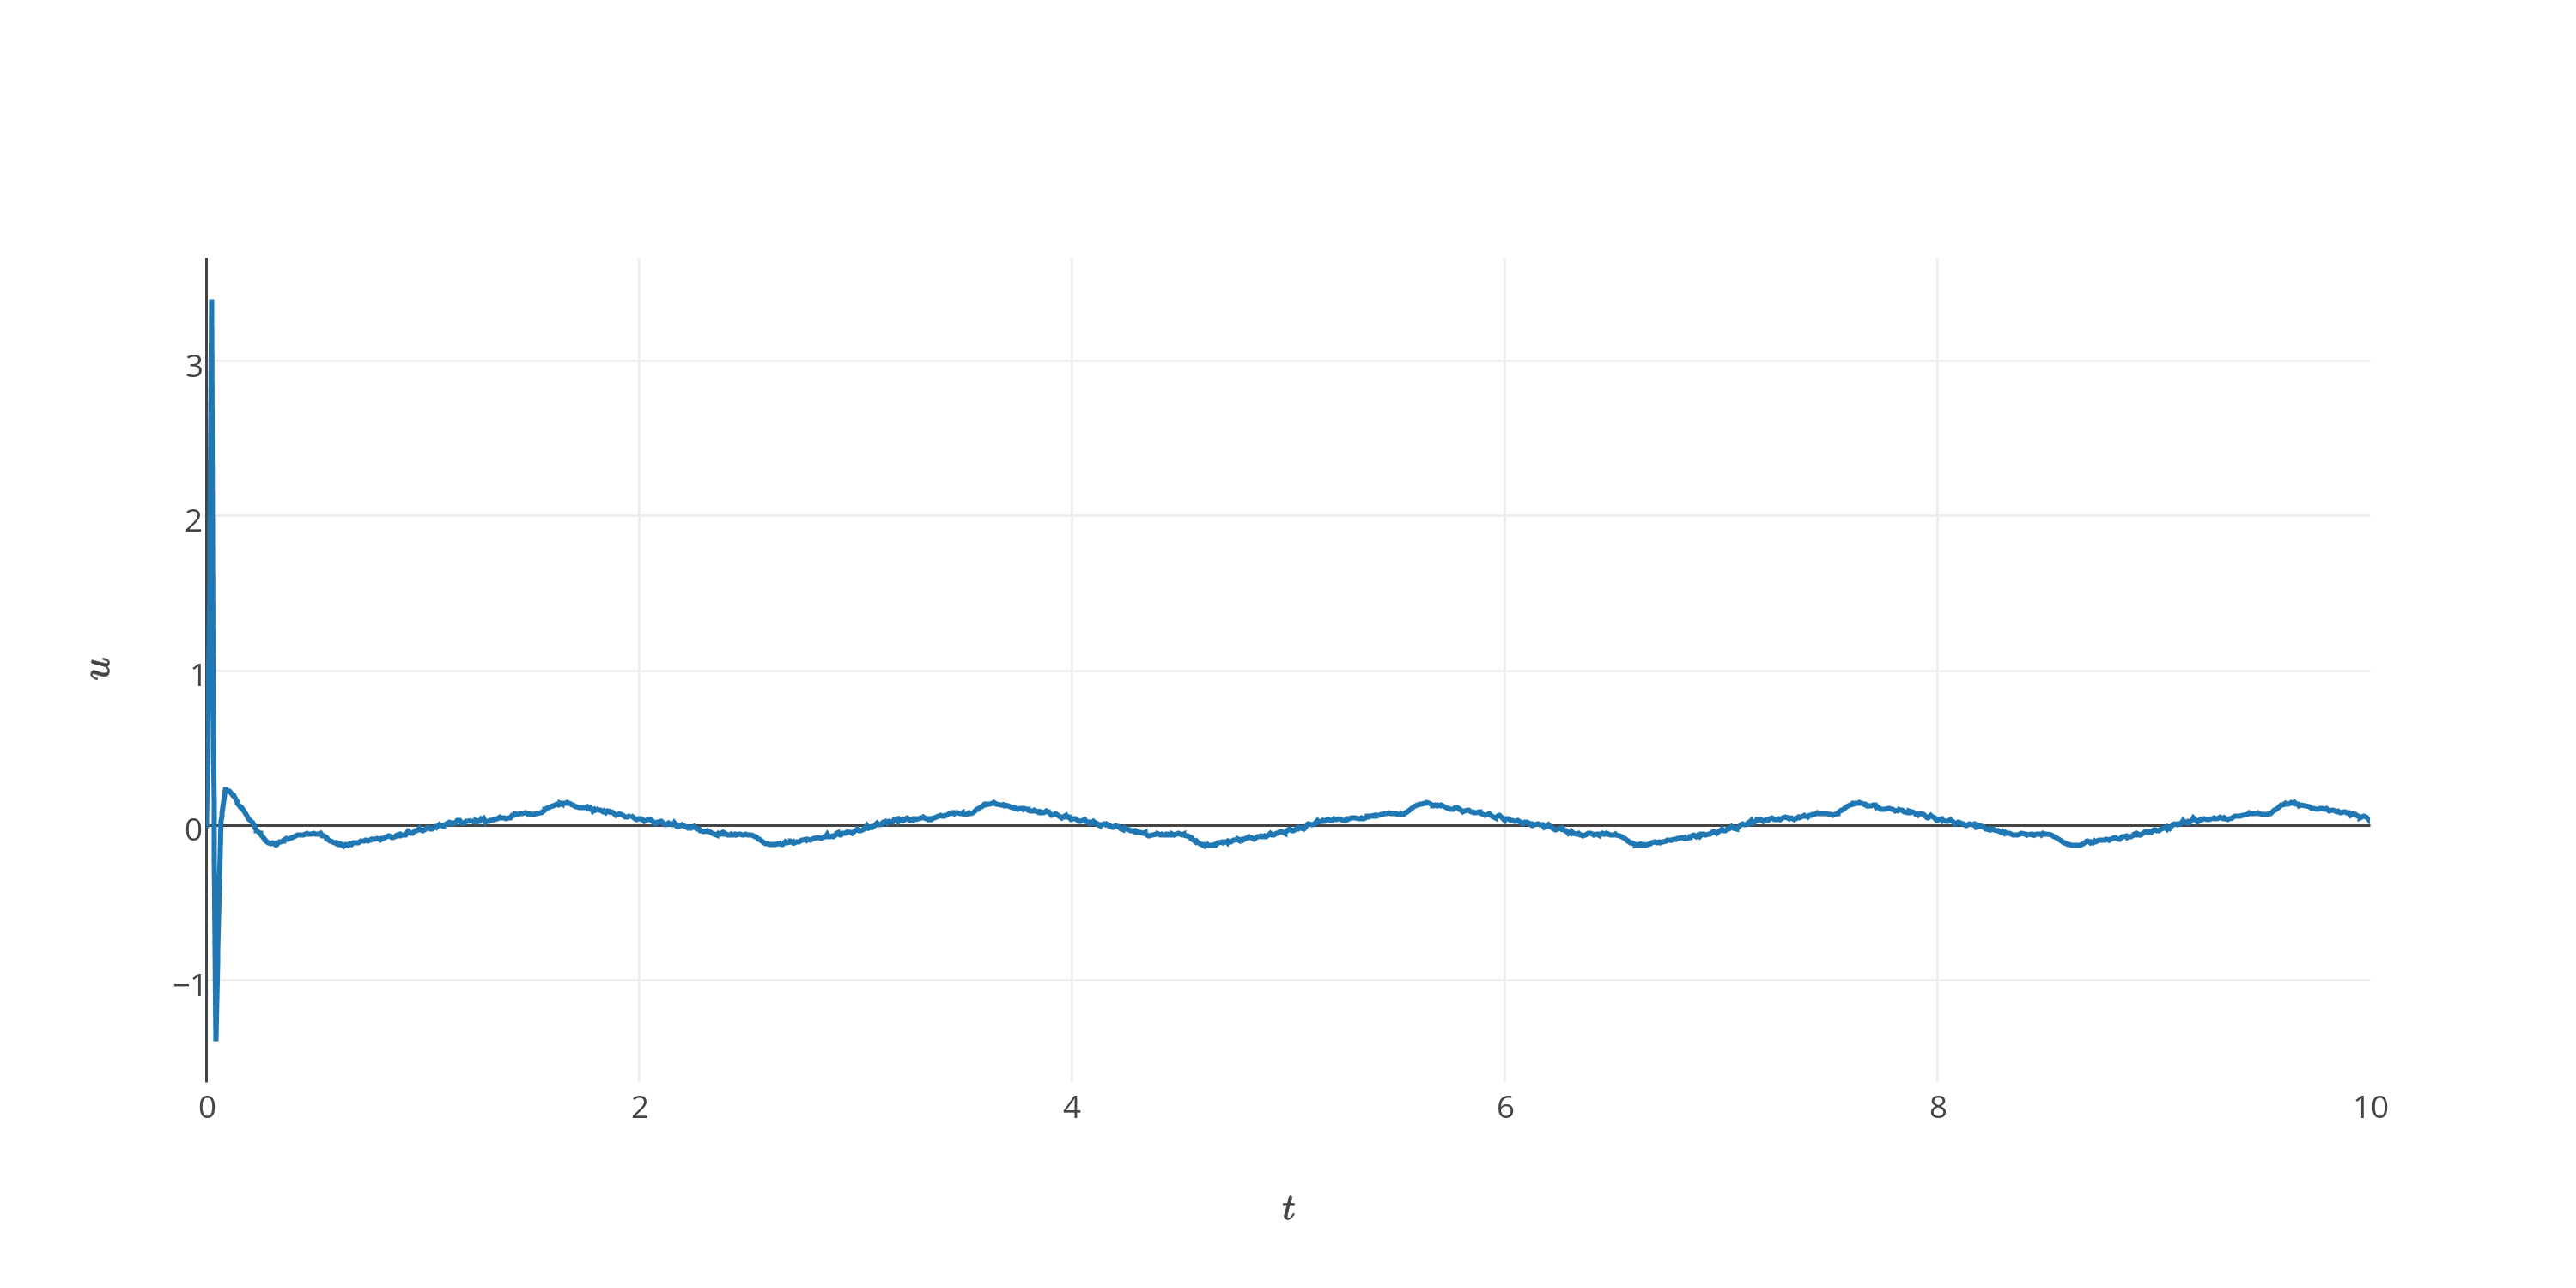
\includegraphics[width=\textwidth]{control}
%     \caption{Control law signal}
%     \label{fig_control}
% \end{figure*}

% Note that IEEE typically puts floats only at the top, even when this
% results in a large percentage of a column being occupied by floats.

% An example of a double column floating figure using two subfigures.
% (The subfig.sty package must be loaded for this to work.)
% The subfigure \label commands are set within each subfloat command,
% and the \label for the overall figure must come after \caption.
% \hfil is used as a separator to get equal spacing.
% Watch out that the combined width of all the subfigures on a 
% line do not exceed the text width or a line break will occur.
%
% \begin{figure*}[!t]
% \centering
% \subfloat[Case I]{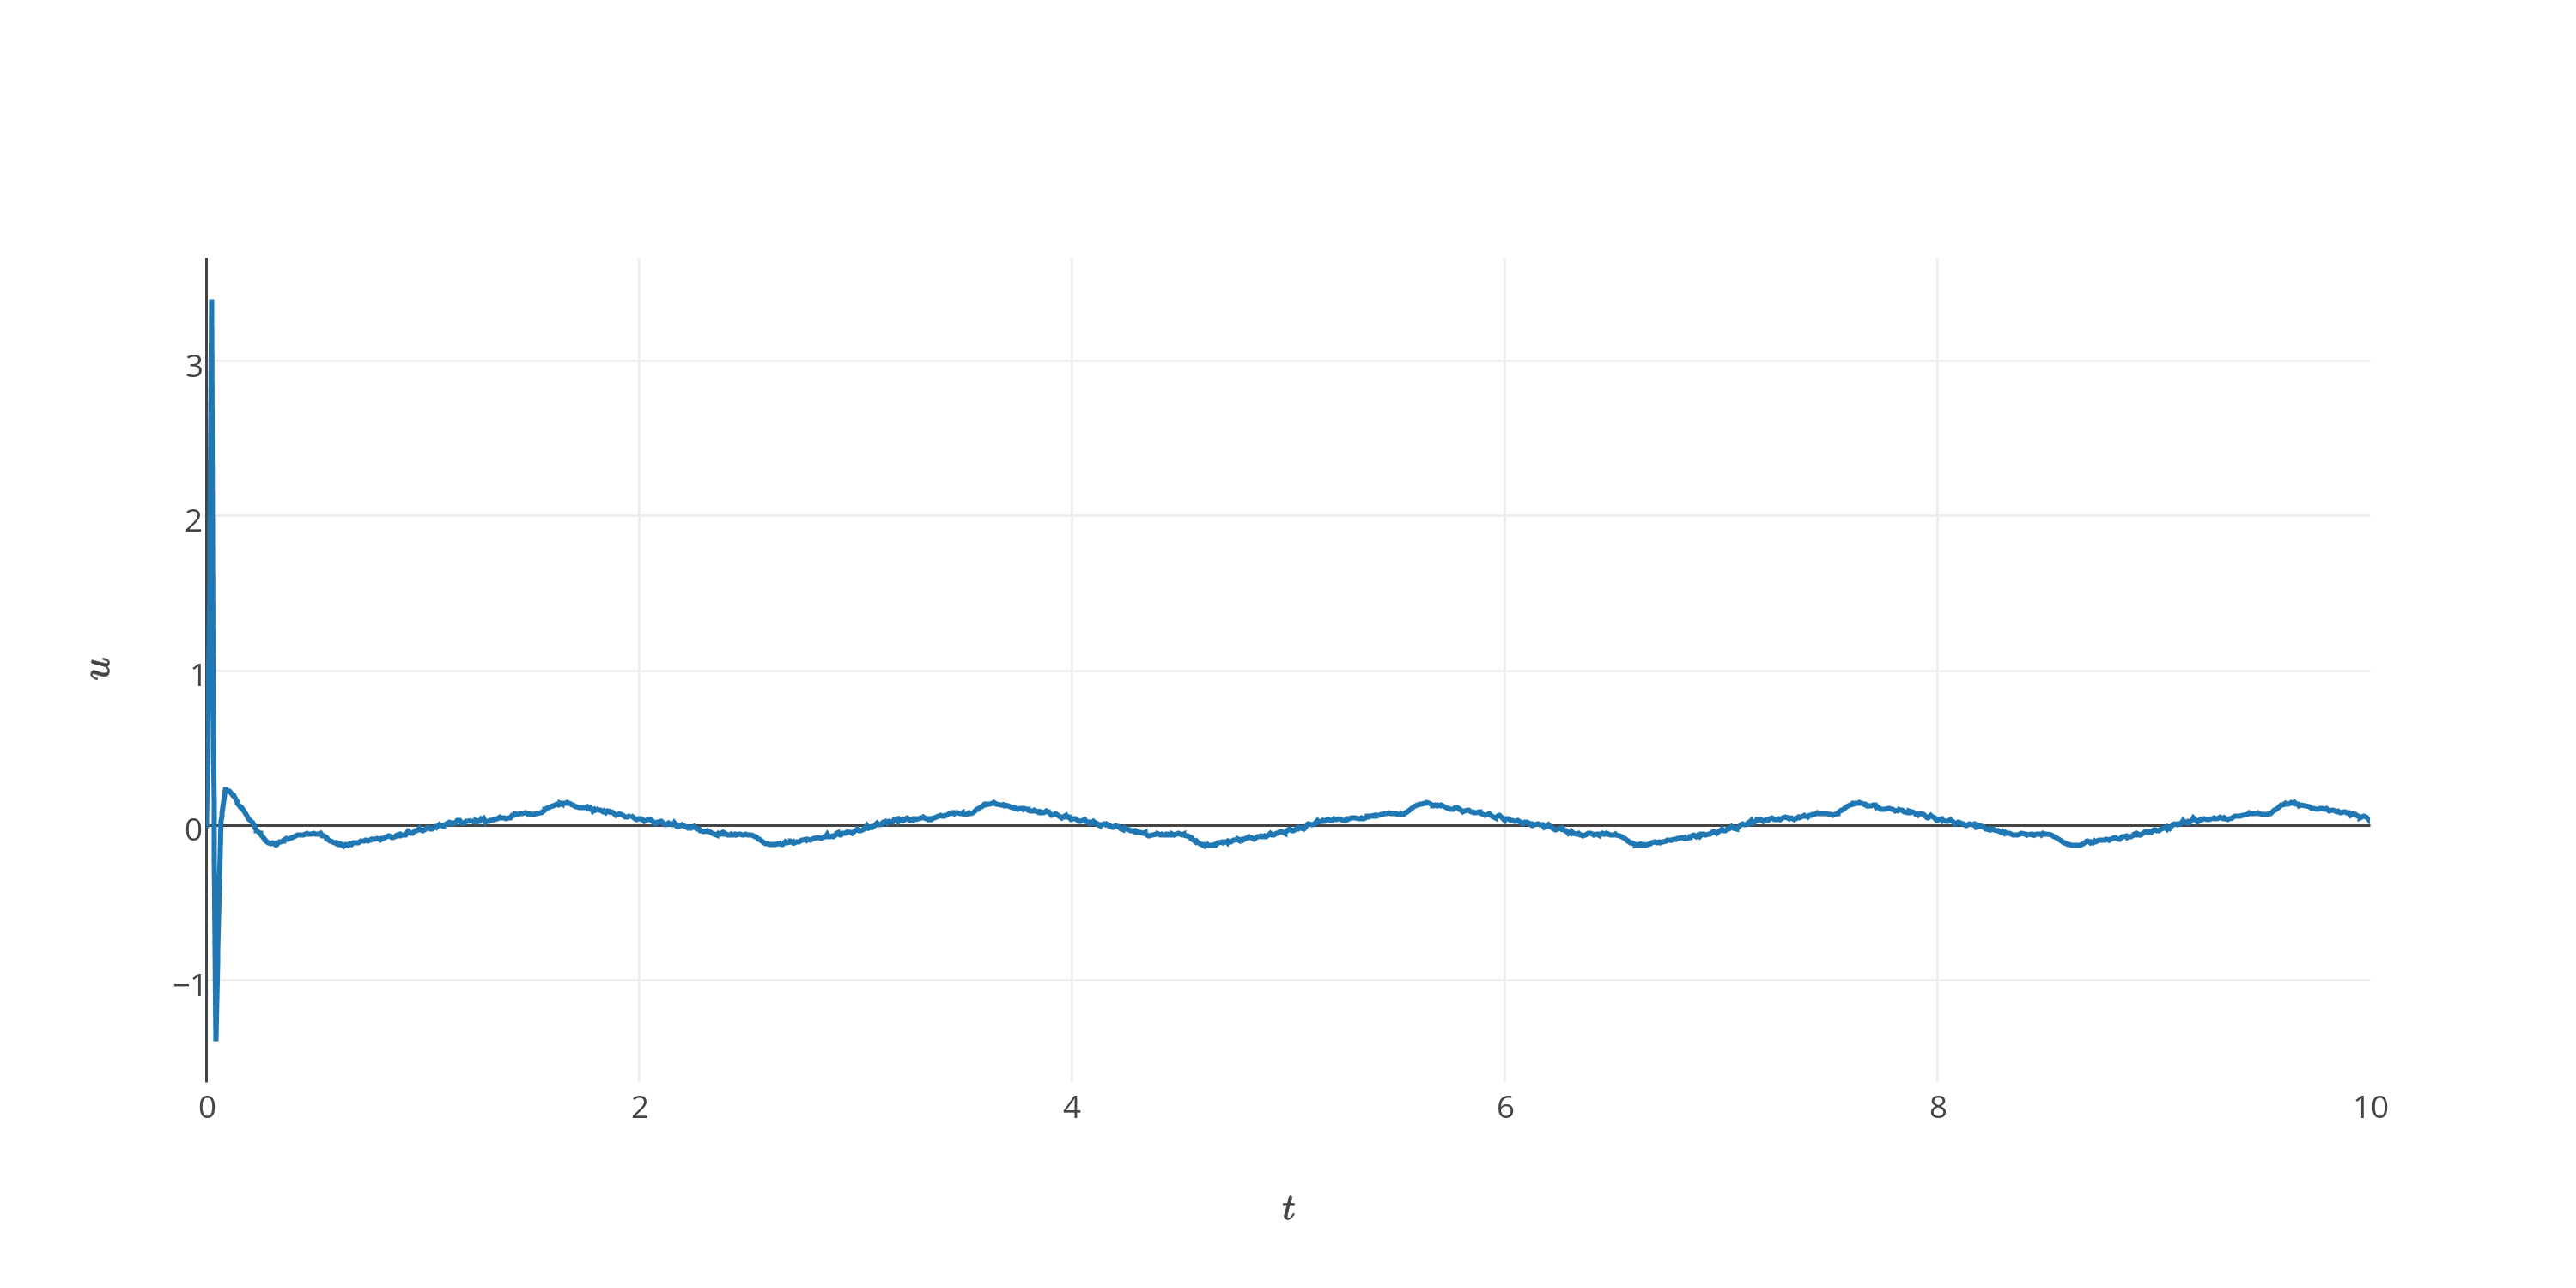
\includegraphics[width=2.5in]{control}%
% \label{fig_first_case}}
% \hfil
% \subfloat[Case II]{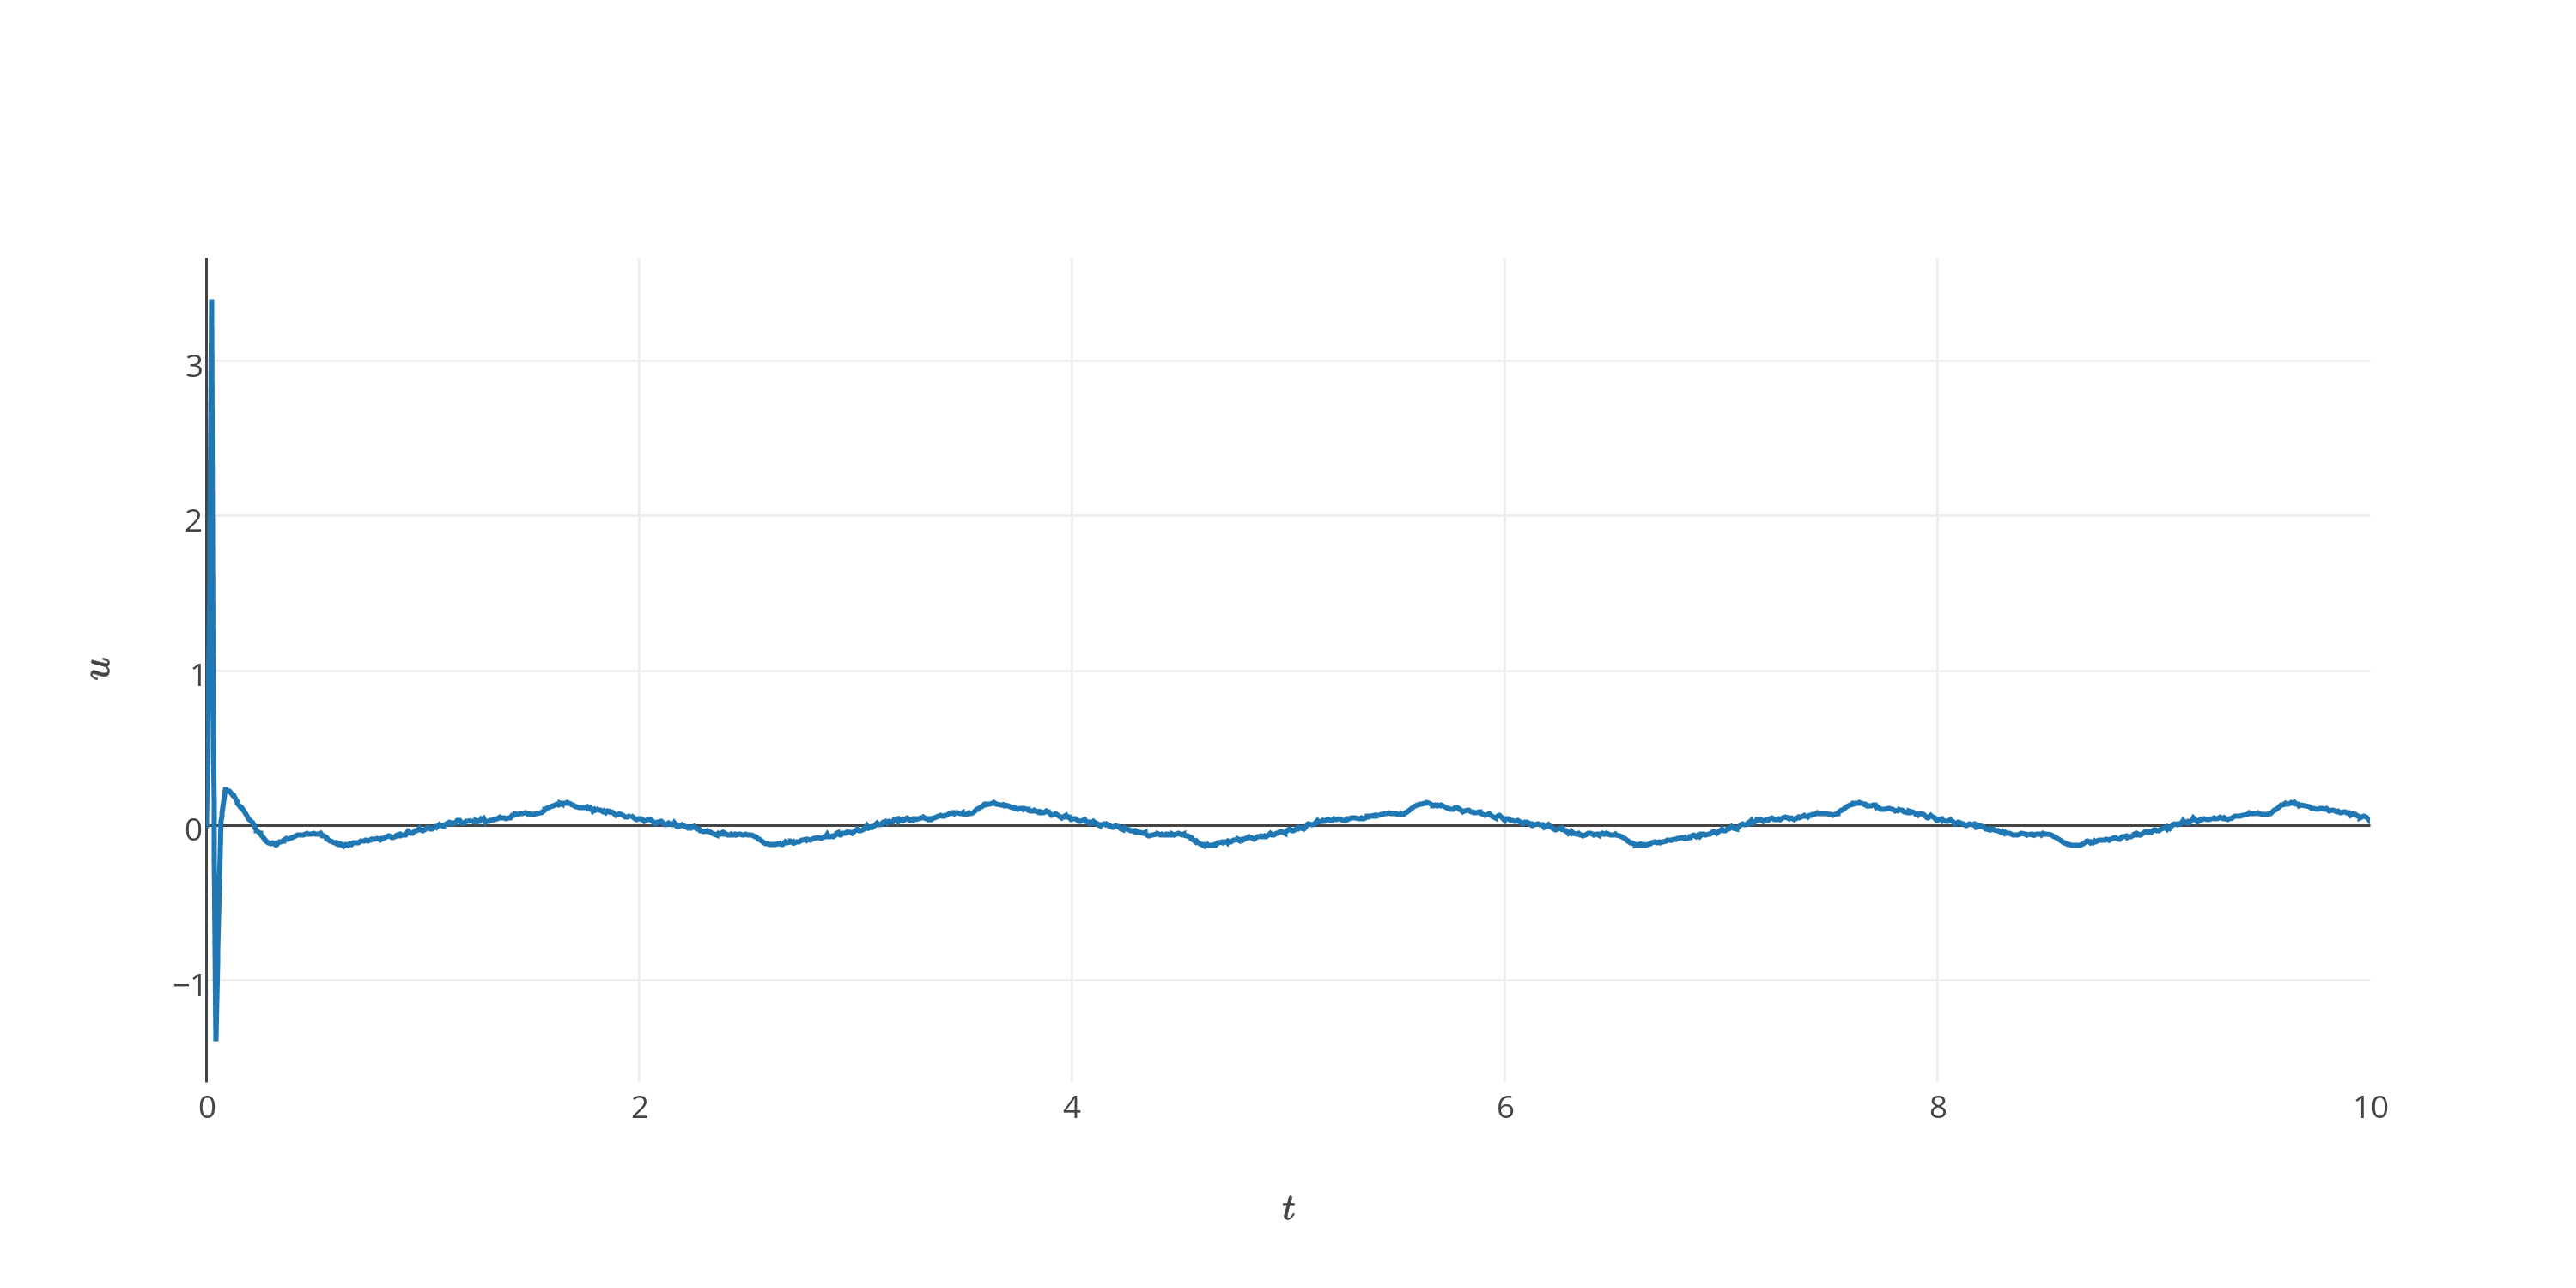
\includegraphics[width=2.5in]{control}%
% \label{fig_second_case}}
% \caption{Simulation results for the network.}
% \label{fig_sim}
% \end{figure*}
%
% Note that often IEEE papers with subfigures do not employ subfigure
% captions (using the optional argument to \subfloat[]), but instead will
% reference/describe all of them (a), (b), etc., within the main caption.
% Be aware that for subfig.sty to generate the (a), (b), etc., subfigure
% labels, the optional argument to \subfloat must be present. If a
% subcaption is not desired, just leave its contents blank,
% e.g., \subfloat[].


% An example of a floating table. Note that, for IEEE style tables, the
% \caption command should come BEFORE the table and, given that table
% captions serve much like titles, are usually capitalized except for words
% such as a, an, and, as, at, but, by, for, in, nor, of, on, or, the, to
% and up, which are usually not capitalized unless they are the first or
% last word of the caption. Table text will default to \footnotesize as
% IEEE normally uses this smaller font for tables.
% The \label must come after \caption as always.
%
%\begin{table}[!t]
%% increase table row spacing, adjust to taste
%\renewcommand{\arraystretch}{1.3}
% if using array.sty, it might be a good idea to tweak the value of
% \extrarowheight as needed to properly center the text within the cells
%\caption{An Example of a Table}
%\label{table_example}
%\centering
%% Some packages, such as MDW tools, offer better commands for making tables
%% than the plain LaTeX2e tabular which is used here.
%\begin{tabular}{|c||c|}
%\hline
%One & Two\\
%\hline
%Three & Four\\
%\hline
%\end{tabular}
%\end{table}

% Note that the IEEE does not put floats in the very first column
% - or typically anywhere on the first page for that matter. Also,
% in-text middle ("here") positioning is typically not used, but it
% is allowed and encouraged for Computer Society conferences (but
% not Computer Society journals). Most IEEE journals/conferences use
% top floats exclusively. 
% Note that, LaTeX2e, unlike IEEE journals/conferences, places
% footnotes above bottom floats. This can be corrected via the
% \fnbelowfloat command of the stfloats package.

\section{Conclusion}
The conclusion goes here.

% if have a single appendix:
%\appendix[Proof of the Zonklar Equations]
% or
%\appendix  % for no appendix heading
% do not use \section anymore after \appendix, only \section*
% is possibly needed

% use appendices with more than one appendix
% then use \section to start each appendix
% you must declare a \section before using any
% \subsection or using \label (\appendices by itself
% starts a section numbered zero.)
%

\appendices
\section{Proof of the First Zonklar Equation}
Appendix one text goes here.

% you can choose not to have a title for an appendix
% if you want by leaving the argument blank
% \section{}
% Appendix two text goes here.

% use section* for acknowledgment
% \section*{Acknowledgment}
% The authors would like to thank...

% Can use something like this to put references on a page
% by themselves when using endfloat and the captionsoff option.
% \ifCLASSOPTIONcaptionsoff
%   \newpage
% \fi

% trigger a \newpage just before the given reference
% number - used to balance the columns on the last page
% adjust value as needed - may need to be readjusted if
% the document is modified later
%\IEEEtriggeratref{8}
% The "triggered" command can be changed if desired:
%\IEEEtriggercmd{\enlargethispage{-5in}}

% references section

% can use a bibliography generated by BibTeX as a .bbl file
% BibTeX documentation can be easily obtained at:
% http://www.ctan.org/tex-archive/biblio/bibtex/contrib/doc/
% The IEEEtran BibTeX style support page is at:
% http://www.michaelshell.org/tex/ieeetran/bibtex/
%\bibliographystyle{IEEEtran}
% argument is your BibTeX string definitions and bibliography database(s)
%\bibliography{IEEEabrv,../bib/paper}
%
% <OR> manually copy in the resultant .bbl file
% set second argument of \begin to the number of references
% (used to reserve space for the reference number labels box)

\newpage

\begin{thebibliography}{1}

\bibitem{IEEEhowto:kopka}
H.~Kopka and P.~W. Daly, \emph{A Guide to \LaTeX}, 3rd~ed.\hskip 1em plus
  0.5em minus 0.4em\relax Harlow, England: Addison-Wesley, 1999.

\end{thebibliography}

% biography section
% 
% If you have an EPS/PDF photo (graphicx package needed) extra braces are
% needed around the contents of the optional argument to biography to prevent
% the LaTeX parser from getting confused when it sees the complicated
% \includegraphics command within an optional argument. (You could create
% your own custom macro containing the \includegraphics command to make things
% simpler here.)
%\begin{IEEEbiography}[{\includegraphics[width=1in,height=1.25in,clip,keepaspectratio]{mshell}}]{Michael Shell}
% or if you just want to reserve a space for a photo:

% insert where needed to balance the two columns on the last page with
% biographies
%\newpage

% You can push biographies down or up by placing
% a \vfill before or after them. The appropriate
% use of \vfill depends on what kind of text is
% on the last page and whether or not the columns
% are being equalized.

%\vfill

% Can be used to pull up biographies so that the bottom of the last one
% is flush with the other column.
%\enlargethispage{-5in}

% that's all folks
\end{document}
